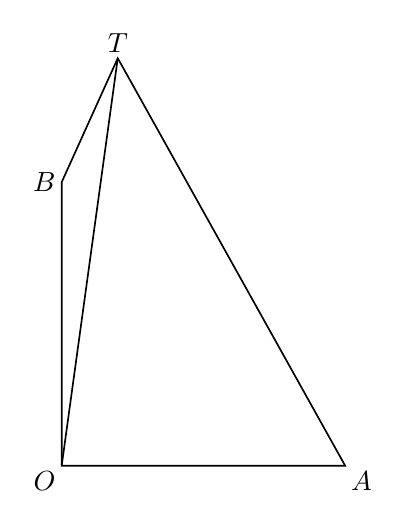
\begin{tikzpicture}[x=1cm,y=1cm,font=\normalsize,
 geometry edge/.style={solid,line width=.6pt},
 geometry mark/.style={solid,line width=.6pt},
 geometry label/.style={font=\normalsize,inner sep=2pt}]
\coordinate (O) at (0.000000000,0.000000000);
\coordinate (A) at (3.600000000,0.000000000);
\coordinate (B) at (0.000000000,3.600000000);
\coordinate (T) at (0.712309500,5.174847000);
\draw[geometry edge] (O)--(A)--(T)--(B)--cycle;
\draw[geometry edge] (O)--(T);
\node[geometry label,below left] at (O) {$O$};
\node[geometry label,below right] at (A) {$A$};
\node[geometry label,left] at (B) {$B$};
\node[geometry label,above] at (T) {$T$};
\end{tikzpicture}
